\begin{frame}{Verificação do Sinal na Bancada}
\begin{columns}[T]
\column{0.49\textwidth}
\centering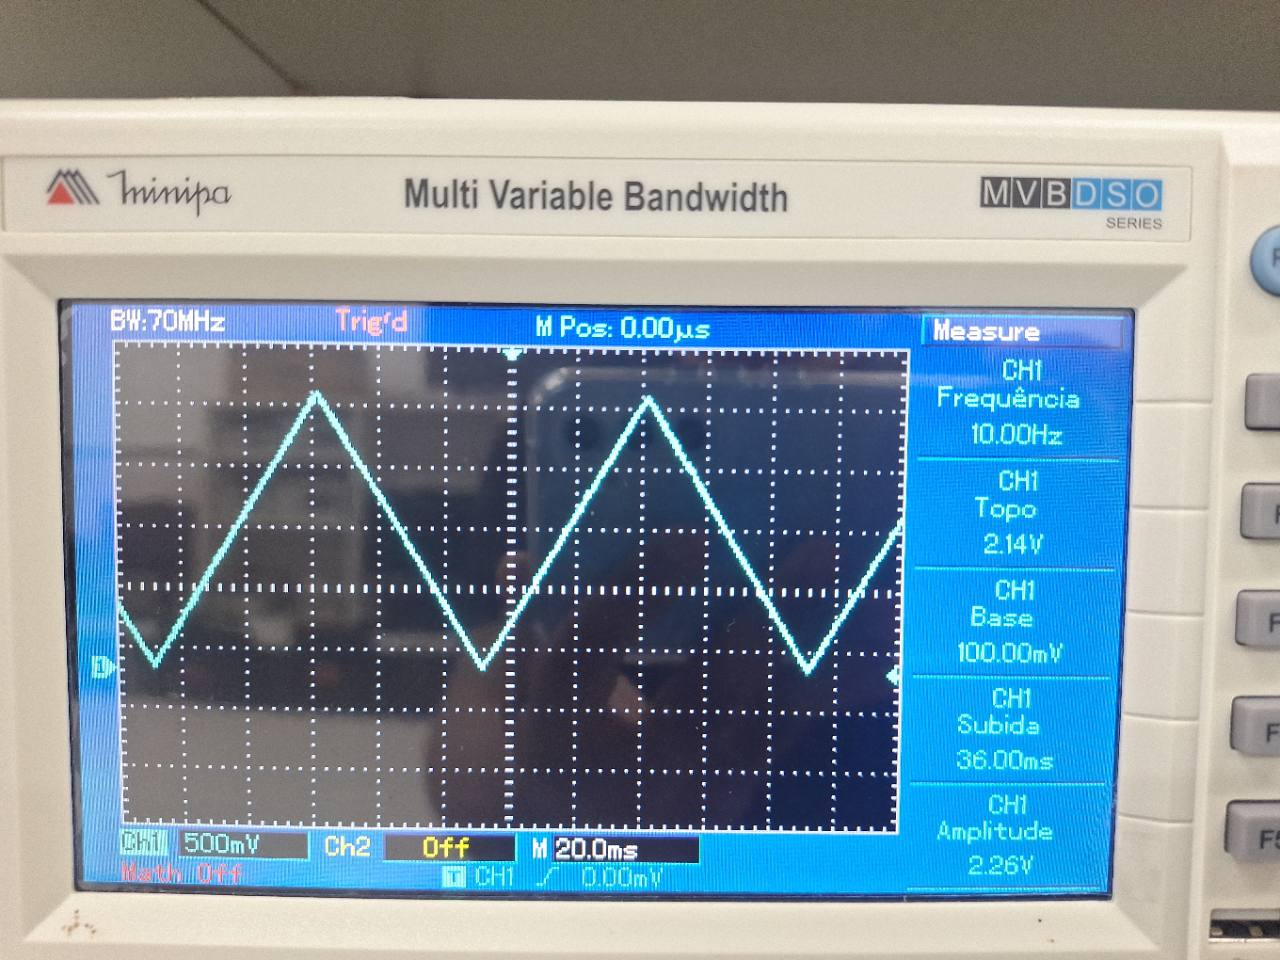
\includegraphics[width=\linewidth]{Imagens/bancada/10hz_sem_arduino.jpg}
\par\small Sem Arduino em paralelo.
\column{0.49\textwidth}
\centering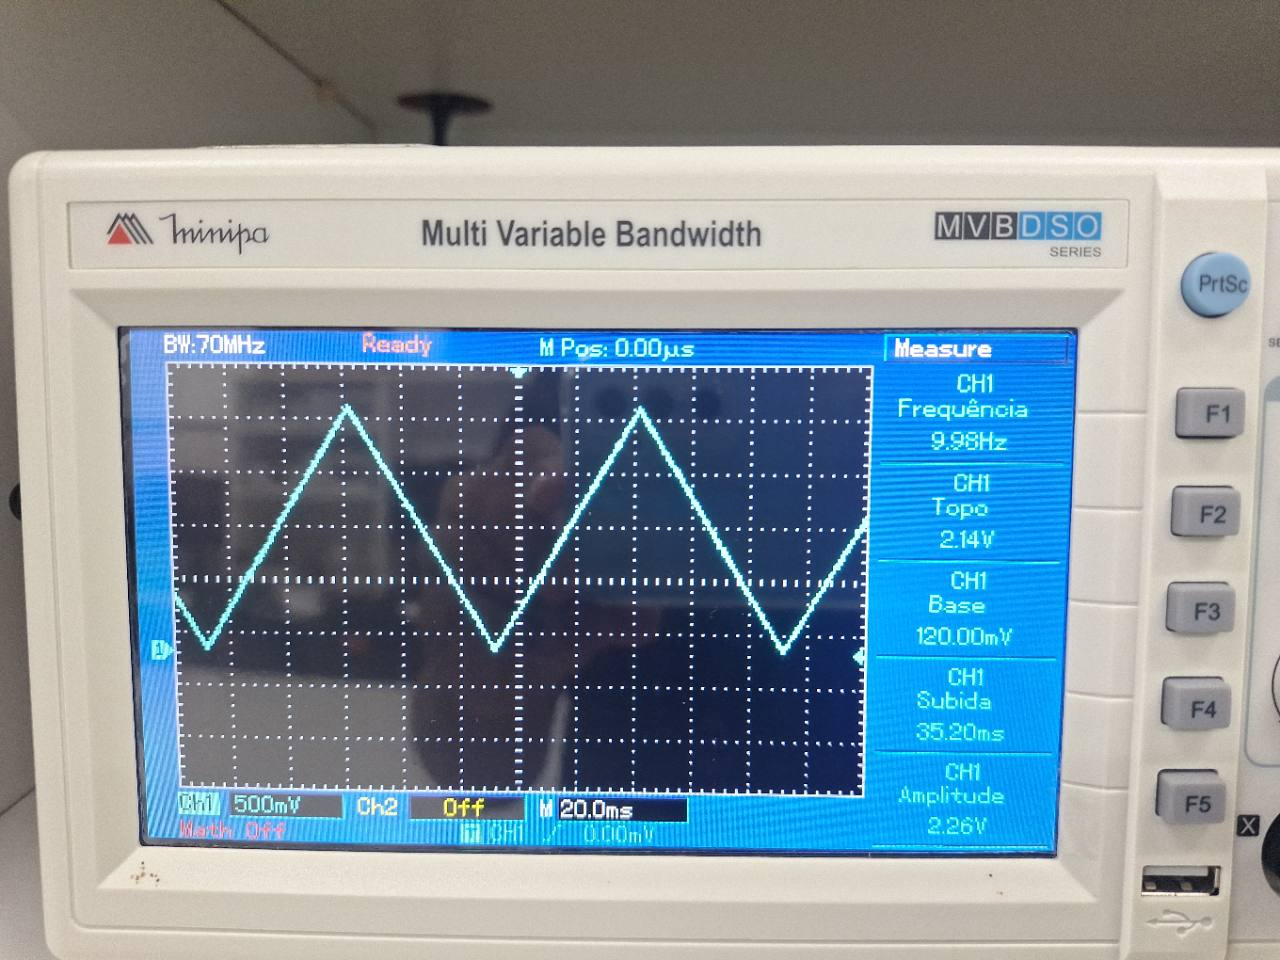
\includegraphics[width=\linewidth]{Imagens/bancada/10hz_com_arduino.jpg}
\par\small Com Arduino em paralelo.
\end{columns}
\begin{itemize}
\item Gerador ajustado em 10 Hz, 2,270 Vpp e offset de 1,145 V.
\item As fotos não mostram mudança expressiva na forma da onda.
\item As medidas automáticas de topo/base não coincidem com os extremos. Por isso, conferimos também máximo, mínimo e pico a pico.
\end{itemize}
\pblfonte{Registros de bancada enviados em 06/11/2026.}
\end{frame}

\begin{frame}{Tensão Medida e Referência do ADC}
\begin{columns}[T]
\column{0.60\textwidth}
\centering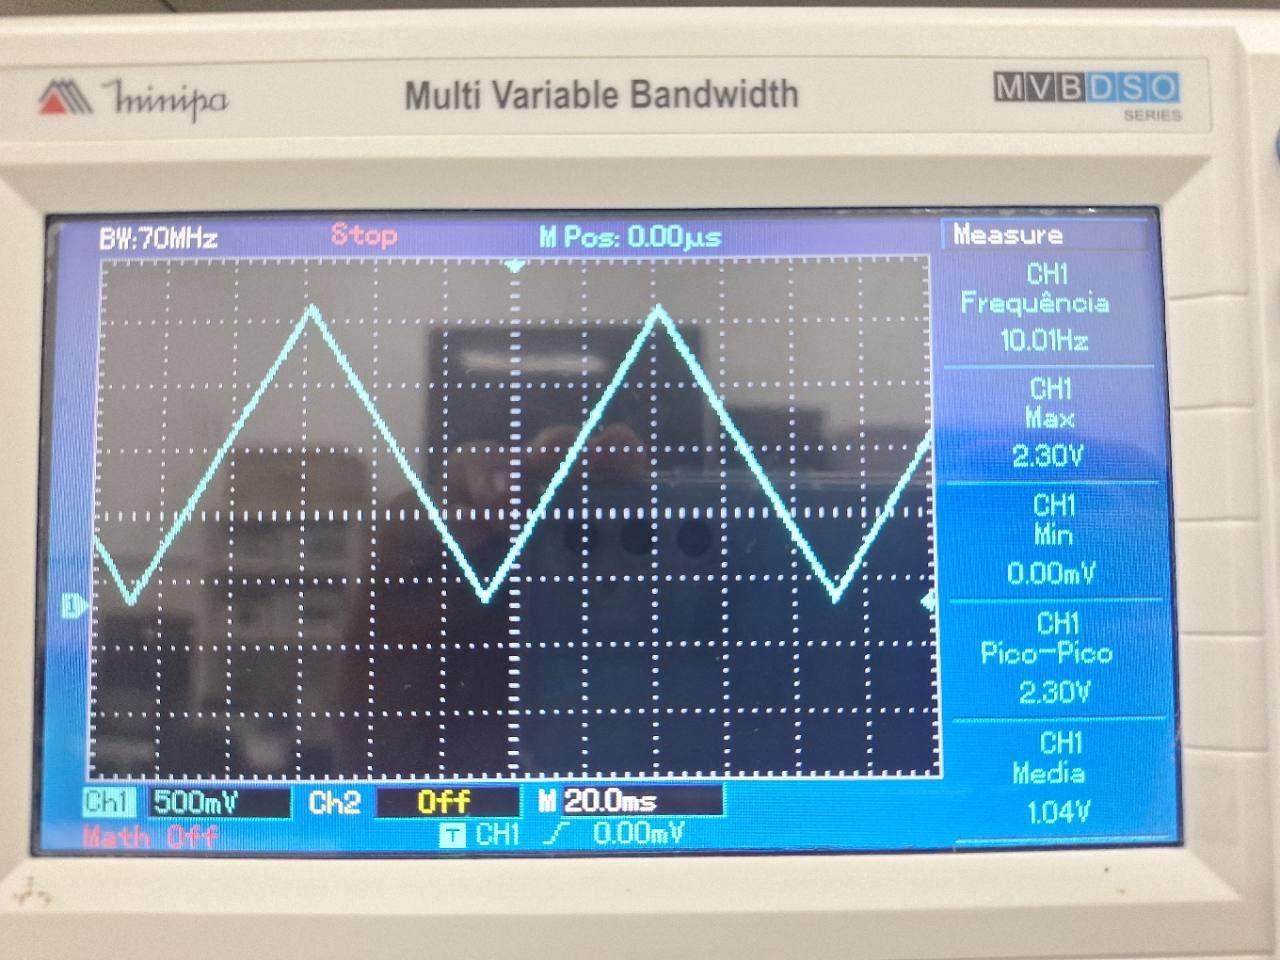
\includegraphics[width=\linewidth,height=4.2cm,keepaspectratio]{Imagens/bancada/10hz_medidas.jpg}
\column{0.36\textwidth}
\small
\begin{tabular}{lr}
$f$ & 10,01 Hz\\
$V_{max}$ & 2,30 V\\
$V_{min}$ & 0,00 V\\
$V_{pp}$ & 2,30 V\\
Média & 1,04 V
\end{tabular}
\par\vspace{0.2cm}
Centro dos extremos: 1,15 V. A média pode variar em uma janela com ciclos incompletos.
\end{columns}
\begin{alertblock}{Escala nominal e medição}
O software usa $V_{ref}=2{,}56$ V. Os 2,30 V medidos e a excursão de 0 a 255 códigos sugerem revisar a escala, mas não calibram a referência.
\end{alertblock}
\pblfonte{Foto de bancada de 06/11; captura digital das 10:28:22.}
\end{frame}

\begin{frame}{Condições da Comparação com o Datasheet}
\small
\begin{tabular}{lrr}
\hline
\textbf{Parâmetro} & \textbf{Tabela 31-9} & \textbf{Ensaio}\\\hline
Resolução de leitura & 10 bits & 8 bits\\
Clock do ADC (erros estáticos) & 200 kHz & 1 MHz\\
Referência (erros estáticos) & 4 V & interna, nominal 2,56 V\\
1 LSB, na mesma referência & $V_{ref}/1024$ & $V_{ref}/256$\\\hline
\end{tabular}
\begin{itemize}
\item Os valores típicos citados nos próximos slides vêm dessa tabela. Não são limites diretamente comparáveis às nossas estimativas em LSB de 8 bits.
\item A edição arquivada informa $V_{INT2}$ entre \textbf{2,4 e 2,8 V} para entrada simples. O limite de 2,3 V aparece na tabela de canais diferenciais.
\item A estimativa de 2,31 V do relatório é uma hipótese de bancada. Precisamos de uma medição independente para avaliar a referência.
\end{itemize}
\pblfonte{Datasheet 2549Q--AVR--02/2014, seção 31.8, tabelas 31-9 e 31-10, pp. 365--367.}
\end{frame}
